\documentclass[11pt, oneside]{article}   	% use "amsart" instead of "article" for AMSLaTeX format
\usepackage{geometry}                		% See geometry.pdf to learn the layout options. There are lots.
\geometry{letterpaper}                   		% ... or a4paper or a5paper or ... 
%\geometry{landscape}                		% Activate for for rotated page geometry
%\usepackage[parfill]{parskip}    		% Activate to begin paragraphs with an empty line rather than an indent
\usepackage{graphicx}				% Use pdf, png, jpg, or eps� with pdflatex; use eps in DVI mode
								% TeX will automatically convert eps --> pdf in pdflatex		
\usepackage{amssymb}

\usepackage{amsmath}

\title{HomeActivity: Recognizing home activities using sensor data}
\author{Stephen Lee, Patrick Pagus and Dong Chen}
%\date{}							% Activate to display a given date or no date

\begin{document}
\maketitle
%\section{}
%\subsection{}
\section{Abstract:}
Home activities recognizing allows many potencial smart applications including healthcare and energy efficiency. In this project, we present the state of the art models for recognizing activities, and show how they performance on the Kasteren-a real world dataset. Comparative analysis metrics including precision, recall, accuracy, F1 mesure and MCC are used in the experiments. Our evaluation results could be used for other pattern recognizing area rather than home activity recognizing.

\section{Introduction}

Activity recognition is the problem of determining an individual's or group's activities given some sensor data describing their actions. More formally, activity recognition finds a function that maps a sequence of sensor readings (feature vectors), to a sequence of activity labels that best describes the sensor data. We focus on activity recognition within home based wireless sensor networks. 

In this case, sensors may include contact, motion, temperature, and humidity sensors located on doors, appliances or monitoring certain rooms. This problem has many applications including healthcare and energy efficiency, where other sensors, such as cameras and wearables, intrude upon privacy or are too expensive or inconvenient. In healthcare, home activity recognition can be used to assess the cognitive and physical capabilities of an elderly person. 

Home energy efficiency can be improved given a schedule of the occupant's activities by scheduling background loads, such as heating, cooling, and various appliances. This domain has several challenges. First, there is a dearth of training data because labeling one's activities is a tedious time consuming process, this limits the number of effective techniques. Second, patterns in training data are specific to the home and the individual. Therefore, the performance of a machine learning technique may vary widely over different data sets. Finally, dominant classes may confound machine learning techniques.

To further our knowledge of machine learning, we will conduct a comprehensive empirical analysis of proposed methods in this domain, across a collection of datasets. These methods include Hidden Markov Models(HMM), Conditional Random Fields(CRF), and Support Vector Machines(SVM). We will apply these methods to at least four datasets that vary in duration, home size, and sensor counts, which are not necessarily proportional to home size. By applying these techniques to real-world datasets and explaining the differences and similarities in their performances, we will gain a deeper understanding of machine learning.

For our group project, we tackle the problem of activity recognition using available sensor information installed in homes. These sensors could be infrared motion detector sensors (to understand when a person entered a room or opened a fridge), to RFID sensors, to microphone based labeling of activities to record the ground truth. These datasets are usually available in the form of timestamp and the corresponding activity or sensor label. So, in this project we would like to predict a label (i.e. the activity) given a sequence of observations. 

\section{Related Works}
Other works show part of the models in their work. It is hard to compare across different works. Instead, we presented a set of models. The evaluation results could be used as the baseline for future research.



The probabilistic models discussed in this chapter represent the state of the art models used in activity recognition. Tapia et al. used the naive Bayes model in combination with the raw feature representation on two real world datasets recorded using a wireless sensor network [16]. HMMs were used in work by Patterson et al. and were applied to data obtained from a wearable RFID reader in a house where many objects are equipped with RFID tags [17]. Wireless sensor network data is more ambiguous than RFID data with respect to activities. For example, when using RFID it is possible to sense which object is used, while with wireless sensor networks only the cupboard that contains the object can be sensed. Because there are usually multiple objects in a cupboard the resulting data is ambiguous with respect to the object used. In work by van Kasteren et al. the performance of HMMs and CRFs in activity recognition was compared on a realworld dataset recorded using a wireless sensor network [18]. Duong et al. compared the performance of HSMMs and HMMs in activity recognition using a laboratory setup in which four cameras captured the location of a person in a kitchen setup [19]. One type of model that we have not included in our comparison are hierarchical models. They have been successfully applied to activity recognition from video data [20], in an office environment using cameras, microphones and keyboard input [21] and on data obtained from a wearable sensing system [22].

\begin{enumerate}
 
\item Interesting because it has applications that spans across various domains:
	\begin{enumerate}
	\item Healthcare\\
		- Long term monitoring of activities could provide us interesting insights on degenerative heath \\
		- Especially useful in monitoring health of elderly people\\
	\item  Energy savings \\
		- Understanding the pattern of activities could help us save energy. \\
		- For example, switching off AC/heater when no one is at home \\
	\item  From a Security perspective\\
		- Again, notifications can be sent to alert the home owners if there is an aberrant activity in the door entrance. \\
	\item  Intelligent Homes\\
		- 
	\end{enumerate}
\item Challenging
		\begin{enumerate}
	\item Sensor datasets could be noisy\\
		- the front doors may open and close multiple times; this doesn't may not indicate that the person has left the home.\\
		- sometimes the sensors itself may have false positives. \\
		
	\item multiple labels may be mapped to a single sensor activity\\
		- opening of a fridge may mean both; make coffee and make cooking\\
		- some other information such as how long the person spent in the kitchen may provide some useful insight\\
		
	\item Imbalanced class problem\\
		- machine learning algorithms and works best when the number of instances of each classes are roughly equal\\
		- where the total number of a class of data (positive) is far less than the total number of another class of data (negative)	\\
		- In this problem, no activity is a perfectly reasonable label. So the prediction model may always output 'no activity' and be accurate 80\% of the time.\\
		\end{enumerate}

\end{enumerate}

\section{Research Problem}

We use more models, compared with other related works.

\section{Recognizing Methods}
We would like to explore the following techniques:
	\begin{enumerate}
\item HMM - 
Hidden Markov Modes (HMM) are a ubiquitous tool for modeling time series data and a generative probabilistic model consisting of a hidden variable and an observable variable at each time step. HMM can be used as black-box density models on sequences. They have the advantage over Markov models in that they can represent long-range dependencies between observations, mediated via the latent variables. 

In our project the hidden variable is the activity performed, and the observable variable is the vector of sensor readings. There are two dependency assumptions: The hidden variable at time t, namely $y_{t}$, depends only on the previous hidden variable $y_{t-1}$. The observable variable at time t, namely $x_{t}$, depends only on the hidden variable $y_{t}$ at that time slice. Then, we can specify an HMM using three probability distributions: the distribution over initial states p($y_{1}$); the transition distribution $p(y_{t}\mid y_{t-1})$ representing the probability of going from one state to the next; and the observation distribution $p(x_{t}\mid y_{t})$ indicating the probability that the state yt would generate observation $x_{t}$.
Learning the parameters of these distributions corresponds to maximizing the joint probability p(x, y) of the paired observation and label sequences in the training data. We can factorize the joint distribution in terms of the three distributions described above as follows:

\begin{equation}
P(x,y)=\prod_{t=1}^{T}p(y_{t}\mid y_{t-1})p(x_{t}\mid y_{t}), p(y_{1}) = p(y_{1}\mid y_{0})
\end{equation}

The parameters that maximize this joint probability are found by frequency counting. Because in our case we are dealing with discrete data, we can simply count the number of occurrences of transitions, observations and states [15]

\item CRF - 
A Conditional Random Field (CRF) is a discriminative probabilistic model that can come in many different forms. The form that most closely resembles the HMM is known as a linear-chain CRF and is the model we use in this project.


\item SVM - 
The implementation used in this experiment comes from SVM

\item SSVM - 

\item Naive Bayes
	\end{enumerate}
The idea of the naive Bayes classifier is to use a generative model of text to estimate


The datasets available to us are:
	\begin{enumerate}
\item Kasteren dataset - has over a month long sensor information from 3 homes.
\item Tulum dataset - more than six month period from a single home
	\end{enumerate}


\section{Experimental Evaluation}

\subsection{Datasets}

The Kasteren dataset is recording a 26-year-old man. He lives alone in a three-room apartment where 14 state-change sensors were installed. Locations of sensors include doors, cup- boards, refrigerator and a toilet flush sensor. Sensors were left unattended, collecting data for 28 days in the apartment. This resulted in 2120 sensor events and 245 activity instances.


\subsection{Experimental Setup}

\subsection{Feather Representation}

 Raw

Changepoint

Last-fired


\subsection{Comparative Analysis Metrics}

\begin{equation}
Precision = \frac{TP}{TP+FP}
\end{equation}

\begin{equation}
Recall = \frac{TP}{TP+FN}
\end{equation}

\begin{equation}
Accuracy = \frac{TP+TN}{TP+TN+FP+FN}
\end{equation}

\begin{equation}
F-Measure = \frac{2\cdot Precision\cdot Recall}{Precison+Recall}
\end{equation}

The Matthews correlation coefficient is used in machine learning as a measure of the quality of binary (two-class) classifications, introduced by biochemist Brian W. Matthews in 1975. It takes into account true and false positives and negatives and is generally regarded as a balanced measure which can be used even if the classes are of very different sizes. The MCC is in essence a correlation coefficient between the observed and predicted binary classifications; it returns a value between −1 and +1. A coefficient of +1 represents a perfect prediction, 0 no better than random prediction and −1 indicates total disagreement between prediction and observation.

\begin{equation}
MCC=\frac{TP\cdot TN-FP\cdot FN}{\sqrt{(TP+FP)\cdot (TP+FN)\cdot (TN+FP)\cdot (TN+FN)}}
\end{equation}


\subsection{Experiments}
\pdfsuppresswarningpagegroup=1
\begin{figure}[t!]
\begin{center}
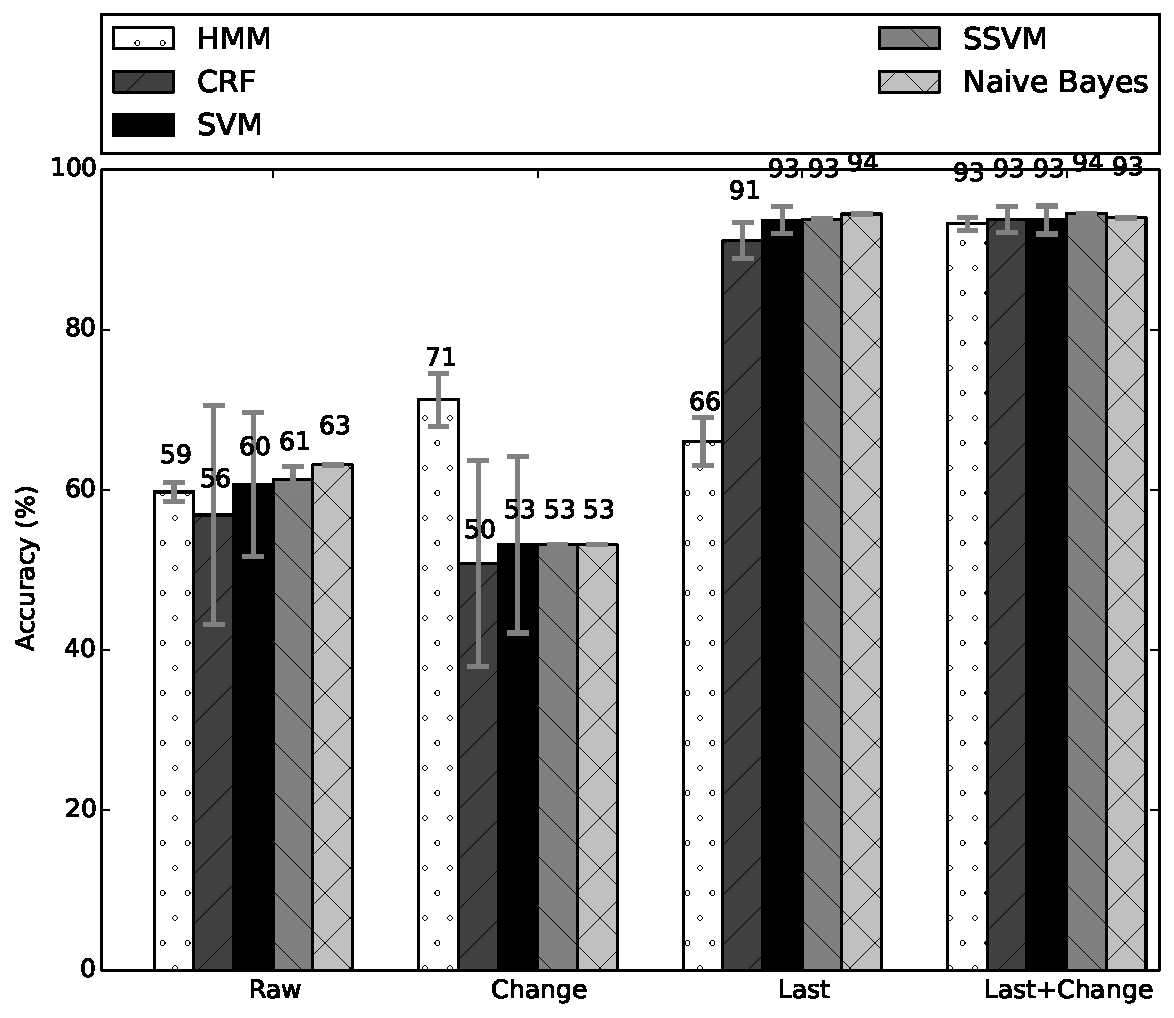
\includegraphics[width=5in]{../../src/reports/A.pdf}
\end{center}
\vspace{-0.5cm}
\caption{House A}
\label{fig:house_a}
\vspace{-0.5cm}
\end{figure}

\begin{figure}[t!]
\begin{center}
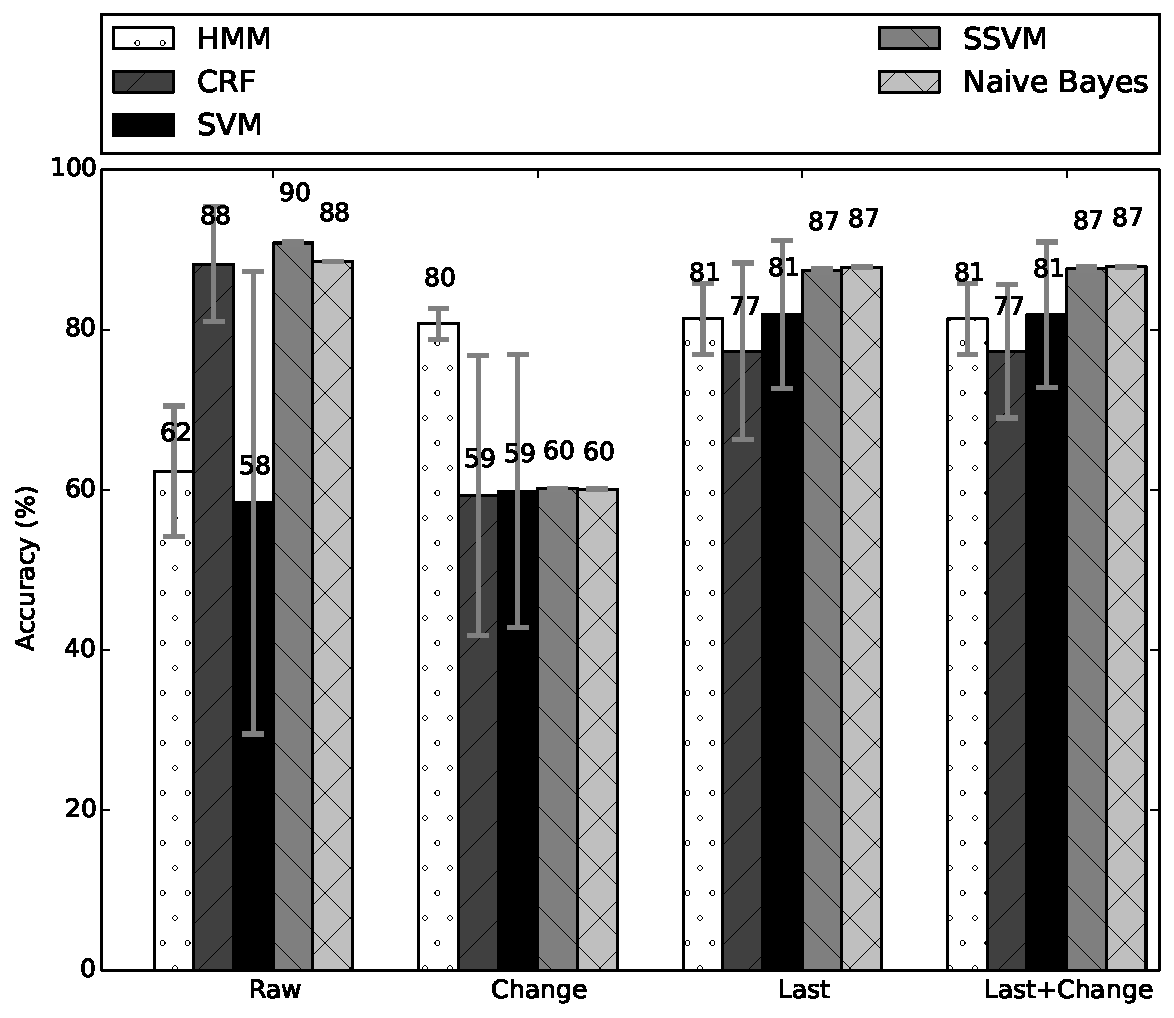
\includegraphics[width=5in]{../../src/reports/B.pdf}
\end{center}
\vspace{-0.5cm}
\caption{House B}
\label{fig:house_b}
\vspace{-0.5cm}
\end{figure}

\begin{figure}[t!]
\begin{center}
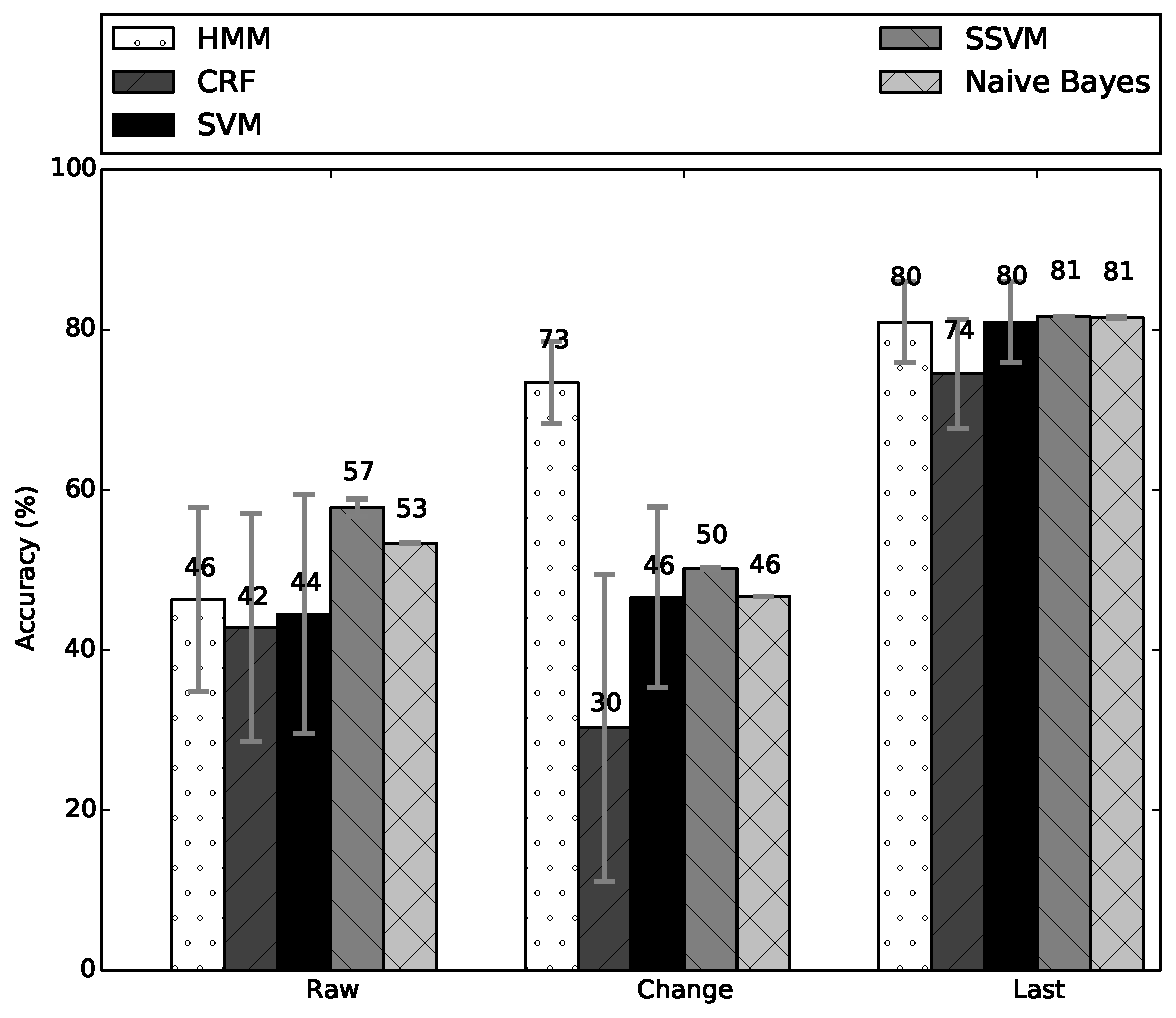
\includegraphics[width=5in]{../../src/reports/C.pdf}
\end{center}
\vspace{-0.5cm}
\caption{House C}
\label{fig:house_3}
\vspace{-0.5cm}
\end{figure}

\section{Discussion and Future Work}


\section{Reference}

\begin{thebibliography}{1}
	
\bibitem{emtapia} E. M. Tapia, S. S. Intille, and K. Larson. {\em Activity recognition in the home using simple and ubiquitous sensors}. In Pervasive Computing, Second International Conference, PERVASIVE 2004, pp. 158–175, Vienna, Austria (April, 2004).

\bibitem{djpatt}  D. J. Patterson, D. Fox, H. A. Kautz, and M. Philipose. Fine-grained activity recognition by aggregating abstract object usage. In ISWC, pp. 44–51. IEEE Computer Society, (2005). ISBN 0-7695-2419-2. URL http://doi.ieeecomputersociety.org/10.1109/ISWC.2005.22.

\bibitem{tvkasteren}  T. van Kasteren, A. Noulas, G. Englebienne, and B. Kro ̈se. Accurate activity recognition in a home setting. In UbiComp ’08: Proceedings of the 10th international conference on Ubiquitous computing, pp. 1–9, New York, NY, USA, (2008). ACM. ISBN 978-1-60558-136-1. doi: http: //doi.acm.org/10.1145/1409635.1409637.

\bibitem{tduong}  T. Duong, D. Phung, H. Bui, and S. Venkatesh, Efficient duration and hierarchical modeling for human activity recognition, Artif. Intell. 173(7-8), 830–856, (2009). ISSN 0004-3702. doi: http://dx.doi.org/10.1016/j.artint.2008.12.005.

\bibitem{sluhr}  S. Luhr, H. H. Bui, S. Venkatesh, and G. A. West, Recognition of human activity through hierarchical stochastic learning, percom. 00, 416, (2003). doi: http://doi.ieeecomputersociety. org/10.1109/PERCOM.2003.1192766.

\bibitem{noliver}  N. Oliver, A. Garg, and E. Horvitz, Layered representations for learning and inferring office activity from multiple sensory channels, Comput. Vis. Image Underst. 96(2), 163–180, (2004). ISSN 1077-3142. doi: http://dx.doi.org/10.1016/j.cviu.2004.02.004.

\bibitem{asubr}  A. Subramanya, A. Raj, J. Bilmes, and D. Fox. Hierarchical models for activity recognition. In IEEE Multimedia Signal Processing (MMSP) Conference, Victoria, CA (October, 2006).


\end{thebibliography}

\end{document}  
